\chapter{Design Intuition for Low Power Energy-harvesting Systems}
\label{chap:intuition}

%There is a rift between industry and research in the way that indoor wireless sensors are powered. Industry has largely eschewed energy harvesting methods, opting instead for the reliability offered by high-density non-rechargeable batteries. 
%Conversely, energy-harvesting is extremely popular for research systems, which have largely abandoned the use of non-rechargeable cells in the pursuit of building systems with indefinite lifetimes. 
%Given this disparity, it is obvious that there is a lack of clarity regarding how wireless sensors should be powered to enable various applications. 
This chapter explores the design space of wireless sensor power supplies. 
The goal of this chapter is to provide high-level guidance for when/if energy harvesting is a beneficial technique instead of, or in addition to, a non-rechargeable storage, how prospective workloads drive component sizing, and if energy-harvesting is utilized, what techniques are required to ensure a minimum useful operation or what is required to maximize energy capture and system reliability. 
This chapter, along with the following chapters, focus on photovoltaic energy harvesting because in indoor conditions, it offers an order of magnitude more energy than other methods.

\section{Formalizing Design Constraints}

The application space for wireless sensors is broad, and very difficult or impossible to enumerate fully. However, there are common application constraints that drive design. By asking a few questions to determine an application requirements, one can begin to describe the design constraints. These questions, in order of their impact on the answers to the other questions, are:
These constraints can be described and parameterized.
In particular, the size, operational lifetime, and harvesting viability 
There are \textit{many} applications that are untenable to enumerate fully. However, they can be described and parameterized by their requirements. An envisioned application can provide constraints on a wireless sensor's size, component selection and sizing, 


%data type quanta vs rate
%reporting rate periodic, reactive

Given a set of application requirements, what are the constraints on the power supply?
\begin{enumerate}
%\item Mobile or static?
\item What size does it have to be?

    $V_{max} = L_{max} * W_{max} * H_{max}$
    
    $V_{primary} + V_{secondary} < V_{max}$
    
\item What are the average power requirements, and what is the largest atomic energy quanta?
    
    $P_{avg, period} = \frac{P_{sleep} * (T_{period} - T_{work}) + P_{work} * T_{work}}{T_{period}}$
    
    Assuming a Poisson distribution over a period $T$:
    
    $P_{avg, reactive} = \frac{P_{sleep} * (T - \lambda * T_{work}) + \lambda * P_{work} * T_{work}}{T}$ 
   
    $P_{avg, intermittent} = P_{harvest}$
    
    $E_{work} = \sum\limits_{e_i\in E} e_i$
    
    $E_{atomic} = \max{E}$
    
    $E_{comms} \in E$
    
    
\item What are the energy storage and lifetime requirements?
    
    $E_{primary} < \rho_{primary} * V_{primary}$
    
    $E_{secondary} < \rho_{secondary} * V_{secondary}$
    
    $E_{secondary} > E_{atomic}$
    
    How to express size of secondary mathematically?
    Energy capacity represents a moving capped sum, is this like a moving average? What is the smallest window that gives us the most return on energy capture?
    At some point, a large enough window allows us to consider the average of harvestable energy, instead of the actual distribution. What is that size?
    
    Given a time series vectors of harvestable and consumed energy of length $N$ 
    
    $E_{trace} = [e_1, e_2, \dots, e_N]$
    $E_{work} =  [w_1, w_2, \dots, w_N]$
    
    at every time, the cumulative energy will be
    
    $ y_0 = \begin{cases} 
        0         & \text{if $e_i - w_i < 0$} \\
        e_i - w_i & \text{if $e_i - w_i > 0$} \\
        E_{secondary} & \text{if $e_i - w_i > E_{secondary}$}
    \end{cases}$
    
    $ y_i = \begin{cases} 
        0             & \text{if $y_{i-1} + e_i - w_i < 0$} \\
        y_{i-1} + e_i - w_i     & \text{if $y_{i-1} + e_i - w_i > 0$} \\
        E_{secondary} & \text{if $y_{i-1} + e_i - w_i > E_{secondary}$}
    \end{cases}$
    
    for an ideal limitless storage:
     
    $ x_0 = \begin{cases} 
        0         & \text{if $e_i - w_i < 0$} \\
        e_i - w_i & \text{if $e_i - w_i > 0$} \\
    \end{cases}$
    
    $ x_i = \begin{cases} 
        0             & \text{if $x_{i-1} + e_i - w_i < 0$} \\
        x_{i-1} + e_i - w_i     & \text{if $x_{i-1} + e_i - w_i > 0$} \\
    \end{cases}$
    
    Unused energy:
    
    $ w_i = x_i - y_i$
    
    $ E_{unused} = \sum_{i=0}^N w_i$
    
    Assuming all energy can be harvested:    

    $E_{h, total} = P_{harvest} * T_{life}$
  
    actual:
   
    $E_{h, actual} = E_{h, total} - E_{unused}$ 
    
    $P_{h, actual} = E_{h, actual} / T_{life}$
    
    
   
    $E_{total} = E_{primary} + E_{h} $
    
    $E_{total} \ge P_{avg} * T_{life}$
    
    $T_{life} = \frac{E_{total}}{P_{avg}}$
    
    
\item How does the average power requirements compare to available harvestable power? 
    
    Energy neutrality:
    
    $P_{h} \ge P_{avg}$ 
    
\item What are the reliability requirements?
\item What are the latency requirements?
\end{enumerate}

\placefigure{fig:intuition:eh_worth_it}
\section{When is Energy-harvesting Worth It?}
This is a question that is often glossed over by energy-harvesting system designers. Many platforms are built under the assumption that energy-harvesting is strictly superior to a primary-only system. 
However, it is important to revisit this question, especially in the context of indoor, low power energy-harvesting. 

\subsection{Power and Energy}
Energy-harvesting is an attractive option for low power designs, as has the potential to supply energy indefinitely. However, that energy is unreliable, and power delivery is limited. Conversely, primary-only systems have a limited amount of energy, but can use that energy at any rate they please, within the power limits of the battery. 
Because of these differences, it can be difficult to directly compare their performance and determine at what scale and in which conditions harvesting is a preferable power source than a primary cell.
Prior work has attempted to approach this comparison with a theoretical cubic sensor of volume $L^3$, with the assumption that the entire sensor volume is dominated by a lithium primary, or the entirety of one $L^2$ face is dominated by a photovoltaic panel.
The authors compare the power provided by the battery cube, with that of the photovoltaic square. 
The energy and power, respectively, provided by a cube of length $L$ is: 

\begin{equation} \label{eqn:intuition:b_energy}
E_b = \rho L^3
\end{equation}
\begin{equation} \label{eqn:intuition:b_power}
P_b = \frac{\rho L^3}{T}
\end{equation}

\noindent Where the energy density $\rho$ is assumed to be 653\si{\milli\Wh\per\cm\cubed}, and $T$ is the lifetime of the battery.
The authors of \cite{yervaGrafting12} assume a 7 year lifetime based on shelf-life in order to calculate the power provided by a primary cell. This assumption very conservative and ignores the impact of sensor workload. 
A more fair estimation for battery lifetime is:

\begin{equation}
T = \frac{\rho L^3}{P_w + P_l}
\end{equation}

\noindent Where $P_w$ is the average power required to drive a sensor workload, and $P_l$ is the self-discharge power of the battery, generally about 1\% a year for a lithium primary battery. Shelf-life effects are not considered, as they are not measurable, and only a manufacturer guarantee. Any aging effects beyond self-discharge are unpredictable. 
With this new definition of battery lifetime, the comparison of power is not as useful a metric, as power provided by the battery is now independent of the battery capacity. 
The power provided by a battery \textit{is} technically limited by its maximum rated load current, which is often related to its capacity. However, this limit is not relevant with low power operation. 
Instead of power, the energy provided to a workload by a primary cell and the energy captured by a similarly sized photovoltaic over the course of the lifetime of the primary cell are directly comparable.

The power provided by a photovoltaic of area $L^2$ is:
\begin{equation}
P_p = \eta E_e L^2
\end{equation}

\noindent 
Where 
$\eta$ denotes the efficiency of the photovoltaic, and is often between 15 and 18\%. 
The spectrial irradiance, $E_e$, is generally between 10 and 100\si{\micro\watt\per\centi\meter\squared} in indoor conditions~\cite{yervaGrafting12,gorlatova2013networking}. 
The authors of \cite{yervaGrafting12} assume the lower end of irradiance, but ignore photovoltaic efficiency.
The amount of energy collected by a photovoltaic over time $T$ is:

\begin{equation}
E_p = \eta E_e L^2 T
\end{equation}

\section{A Framework for Power Supply Design}
\label{sec:framework}
We seek to illustrate the design space for energy-harvesting sensors in two
ways. The first defines an energy-harvesting sensor framework to examine
when designs are feasible and when they require intermittent techniques to make meaningful forward progress.
The second examines dynamic income energy and device behavior through numerical
modeling and simulation.  The framework is based on three key metrics:
harvested energy income, workload, and capacity.
\placefigure{fig:framework}

\subsection{Sensor Regimes}
\label{sec:framework:regime}
The framework splits the design space into four main regimes: always on,
infeasible, checkpointing required, and no intermittent techniques required.
These regimes and their constraints are illustrated in \cref{fig:framework},
and explained in more detail below. \\

\vspace{-6pt}
\noindent
\textbf{Always On.} If the energy harvester supplies a sensor with
more power than the max power it will ever draw, then the device needs
no energy buffer capacity to remain operational. If this is not the case,
then a sensor must have some ability to buffer energy to use when its
operating power exceeds than the harvester input power.
\\

\vspace{-6pt}
\noindent
\textbf{Infeasible.} If the energy harvester supplies less power than
the system leakage, the energy buffer will never
charge. If the energy buffer capacity is less than the
energy required to perform a workload's largest atomic operation, with energy harvested
during the operation itself, then that operation will not have enough energy to
complete.  Neither of these designs will make forward progress and are
therefore infeasible.
Common atomic operations on energy-harvesting sensors include sampling a sensor,
sending a radio packet, booting the processor, and performing a checkpoint.
\\

\vspace{-6pt}
\noindent
\textbf{Checkpointing Required.} If the energy buffer can
hold enough energy to perform atomic operations, but
not enough to complete
workloads composed of multiple, chained
atomic operations (such as sampling a sensor and then sending a radio packet), then
a mechanism for saving state and continuing progress on the next reboot
must be employed.
\\

\vspace{-6pt}
\noindent
\textbf{No Intermittent Techniques.} A sensor that has enough harvester
potential and energy capacity to complete a workload's longest non-atomic
operation can operate without checkpointing. Such systems also benefit as
energy devoted to checkpointing can be used for a workload instead.
\\

\vspace{-6pt}
\noindent
\textbf{Hysteresis Management.}
Finally, if a sensor's deep sleep power draw %willfully powers down
is a substantial fraction of the harvester power, as
is the case with Capybara~\cite{colinReconfigurable18}, then it is
beneficial to continue operating until the energy
buffer is depleted, power off, and recharge quickly
rather than stop early and recharge slowly.
Under this scenario, hysteresis management techniques,
such as reconfigurable capacity and federated energy can increase sensor
performance as discussed in \cref{sec:related}.
The utility of hysteresis management is diminished
when the ratio of harvester power to deep sleep power increases.
For sensors that can willfully power off or sleep,
operating thresholds can be controlled, disentangling
capacity and charging hysteresis.
Their deep
sleep power is equal to leakage, and such techniques
will not improve recharge times.

For all systems, these techniques can decrease cold start time
by reducing the capacity that must be charged
to achieve cold start.

This is more beneficial for systems that cold start frequently and
have a higher energy capacity, however,
a higher-capacity energy store also has a lower probability of
needing to cold start. Therefore the benefits of hysteresis management for
cold start with respect to storage capacity are in conflict with their necessity,
and we do not attempt to quantify these subtle nuances in \cref{fig:framework}.

\subsection{Framework Limitations}
\label{sec:framework:limitations}
This framework makes a couple simplifying assumptions that prevent it from
fully capturing the richness of the design space.\\

\vspace{-6pt}
\noindent
\textbf{Backup Energy Store.}
This framework does not consider the impact of a backup energy store.
%that is pre-charged before the sensor begins operation.
%The simplest way
%to view
A backup energy store can be viewed as the ability to inject additional energy
to the system at arbitrary times,
%move the system
%outside of the regime of requiring checkpoints for very energy intensive operations, or
eliminating the need for checkpointing when there is very low
harvesting potential.

A backup energy store could also contribute in more subtle ways. It could
allow a system to avoid the energy and complexity of checkpointing by
providing just enough energy for a deep sleep mode with state retention rather
than a full power down when the system depletes its stored energy. It could also
cold start energy buffer charging to eliminate the need for reconfigurable
power supplies, or to increase the efficiency of
the energy-harvesting front-end at low voltages.
Finally, in periods of long energy drought, the backup energy store could increase
sensor availability.

While the use of a backup energy store
does constrain the sensor to a finite lifetime,
%especially since current technology favors non-rechargeable, primary-cells as
%backup energy stores,
energy-harvesting can substantially extend these lifetimes under certain harvesting
conditions.\\
%We explore the lifetime of energy-harvesting
%designs with backup energy stores in \cref{sec:primary}.

\vspace{-6pt}
\noindent
\textbf{Constant Harvester Power.}
The framework assumes an energy harvester will supply a constant energy
income, when in reality income is often highly variable. In practice, a sensor
platform both defines the regions of the plot, and occupies a
vertical line which represents the energy storage capacity of the sensor
combined with the range of harvester input powers it might experience. We expect
this line will span multiple regions for most sensors.

However, by ignoring variability, the plot also fails to illustrate key benefits
of capacity under varying energy incomes and workloads. Intuitively,
higher energy buffer capacity can store energy in times of excess and supply
that energy in times of drought. This balancing out of energy income
effectively raises the minimum power supplied by the energy harvester.
Because the extent of this impact is completely dependent on the variability
of the energy income and workload of the sensor, we also develop a numerical simulation to
quantify the impact of capacity
on key metrics including energy utilization, availability and reactivity.

\section{An Intuitive Case for Capacity}

\begin{definetable}{tab:related}
  \scriptsize
  \begin{threeparttable}
  \centering
  \begin{tabular}{l | c c| c c| c}
      \multirow{2}{*}{Platform} & \multicolumn{2}{c|}{Successful Events\,(\%)}  & \multicolumn{2}{c|}{\parbox{2.5cm}{\centering Long-Running\\Time to Completion Ratio}} & \multirow{2}{*}{Lifetime\,(yrs)}\\
                              & Periodic     & Reactive                     & Average & 95th Percentile & \\
    \hline
    Telos \cite{polastre2005telos}                      & 100   & 100   & 1     & 1     & 8.55\\
    Hamilton \cite{kim2018system}                & 100   & 100   & 1     & 1     & 6.75\\
    BLEES \cite{adkins2015michigan}                     & 100   & 100   & 1     & 1     & 1.11\\
    Gecko \cite{yervaGrafting12}                 & 39.5  & 64.9  & 387   & 981   & $\infty$\,\tnote{g} \\
    Capybara~\cite{colinReconfigurable18}\,\tnote{a}    & 46.3  & 72.8  & 37.6  & 1     & $\infty$\,\tnote{g}\\
    Capybara~\cite{colinReconfigurable18}\,\tnote{b}    & 41.1  & 67.1  & 2730  & 8900 & $\infty$\,\tnote{g}\\
    Flicker \cite{hesterFlicker17}                      & 39.3  & 64.2  & 1307  & 5670 & $\infty$\,\tnote{g}\\
    EnHANTs \cite{margolies2015energy}                  & 79.4  & 96.0  & 1     & 1     & \textemdash\,\tnote{h}\\
    DoubleDip \cite{martin2012doubledip}                & 77.9  & 66.5  & 1     & 1     & \textemdash\,\tnote{h}\\
    \cite{raisigel2010autonomous}                       & 78.4  & 66.9  & 1     & 1     & \textemdash\,\tnote{h}\\
    \textbf{\name}\,\tnote{c}                           & 81.2  & 98.3  & 1     & 1     & \textemdash\,\tnote{i}\\
    \textbf{\name}\,\tnote{d}                           & 100   & 100   & 1     & 1     &  35.8\\
    \textbf{\name}\,\tnote{e}                           & 100   & 100   & 1     & 1     &  30.2\\
    \textbf{\name}\,\tnote{f}                           & 100   & 100   & 1     & 1     &  6.27\\
  \end{tabular}
    \begin{tablenotes}[para]
      \item[a] With capacitors: 400\,\si{\micro\farad} ceramic + 330\,\si{\micro\farad} tantalum + 67.5\,mF supercapacitor.
      \item[b] With capacitors: 300\,\si{\micro\farad} ceramic + 1100\,\si{\micro\farad} tantalum + 7.5\,mF supercapacitor.
      \item[c] No primary-cell.
      \item[d] AA primary-cells like Telos.
      \item[e] CR123A primary-cell like Hamilton.
      \item[f] CR2032 like BLEES.
      \item[g] Lifetimes are theoretically infinite for capacitor-based systems.
      \item[h] Not enough information to predict cycling failure time for theses systems.
      \item[i] Expect cycling failure in 20-50 years, but do not attempt to estimate.
    \end{tablenotes}
  \end{threeparttable}
  \caption{
  \normalfont
      Modeled performance of energy-harvesting systems.
    For each  platform considered, we model the performance of its energy storage
    architecture. Periodic workload and lifetime estimates are based on a 10\,s
    period, and the reactive workload is scaled to
    generate a maximum of 2000 events per hour (3.4\,s average daily period). Generally,
    intermittent systems have significantly worse availability and responsiveness compared to
    battery-only systems and systems that use a secondary-cell. Battery-only
    systems achieve perfect operation, but have finite, sub-decade lifetimes.
    }
\end{definetable}

\begin{definefigure}{fig:framework}
  \centering
  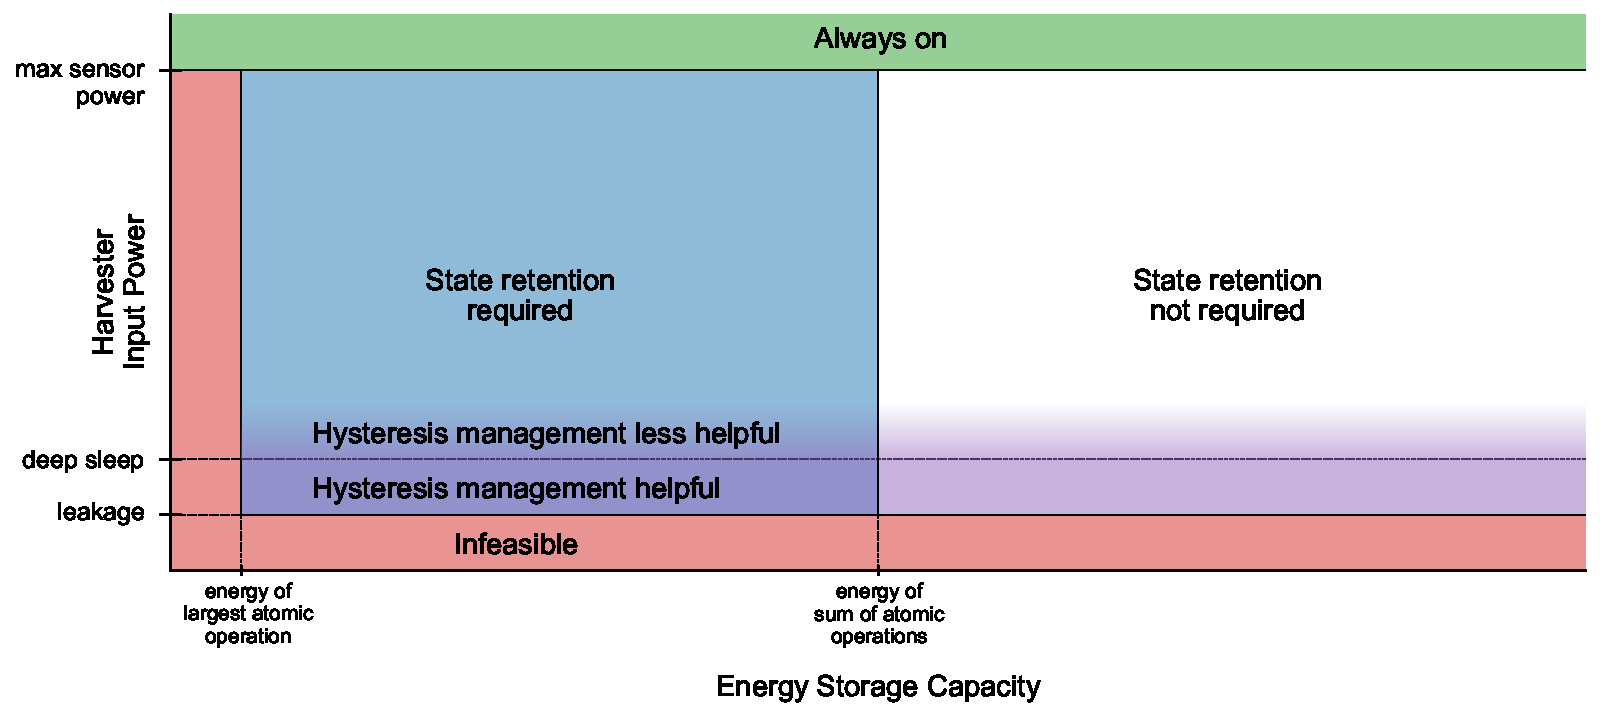
\includegraphics[width=\columnwidth]{figs/capacity/harvesting_framework/framework}
  \caption{
  %energy-harvesting
  %sensors have different capabilities and requirements
  \normalfont Design space for energy-harvesting sensors based on their energy
  income (which we assume is constant for this analysis), energy storage capacity, and workload.
  Workload is represented by the largest atomic/non-atomic operations supported
  by a design, as well as the deep sleep and leakage power.  The plot breaks
  into four regions: \textbf{1)} always
  on or effectively powered, \textbf{2)} Infeasible due to lack of energy storage or
  leakage higher than harvesting rate \textbf{3)} Feasible but requires checkpointing
  to make forward progress, and \textbf{4)} Enough energy storage to not require
  or benefit from checkpointing. Additionally, sensors which have high
  power when they enter deep sleep before depleting their
  energy buffer may benefit from hysteresis management techniques.
  This benefit diminishes with lower sleep currents and higher harvesting potential.
  %With increased capacity, sensors can avoid the complexity of intermittent
  %programming techniques and specialized, reconfigurable power supplies in addition
  %to the other benefits of increased capacity discussed
  %in \cref{sec:store}.
  }
\end{definefigure}


\begin{definefigure}{fig:intuition:eh_worth_it}
  \centering
  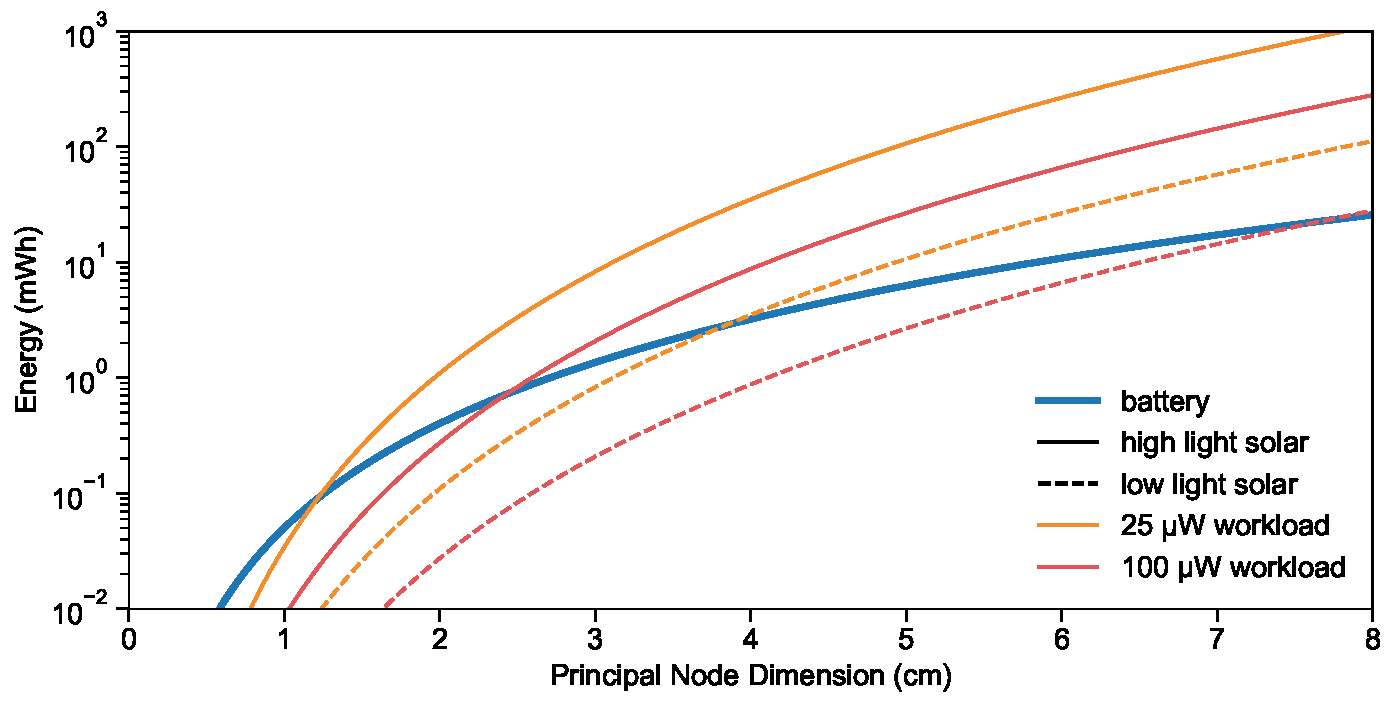
\includegraphics[width=\columnwidth]{figs/is_eh_worth_it.pdf}
  \caption{
  An updated energy-harvesting reality check~\cite{yervaGrafting12}. This figure compares the energy offered by a battery with that of potential harvestable energy over the lifetime of the same battery. Assuming a cubic sensor, driven by a  principal dimension $L$, a battery of size $L^3$ provides a lifetime of $T$, under different average workloads, here represented by the orange (average 25\si{\micro\watt}) and red (100\si{\micro\watt}). 
  A solar cell of size $L^2$ accumulates energy over that same lifetime $T$, and if large enough and in sufficient harvesting conditions, will exceed that of a similar sized battery, albeit only in 2 dimensions.  The point at which the harvesting lines (orange, red) cross the battery line (blue) indicate the size at which a solar panel of size $L^2$ will harvest the same amount of energy provided by a battery of size $L^3$ over its lifetime. At a sufficient size and in sufficient harvesting conditions, while powering an appropriate workload, solar energy-harvesting can provide more energy over the same time frame as a lithium battery.
  }
\end{definefigure}

\begin{definefigure}{fig:intuition:primary+harvesting}
  \centering
  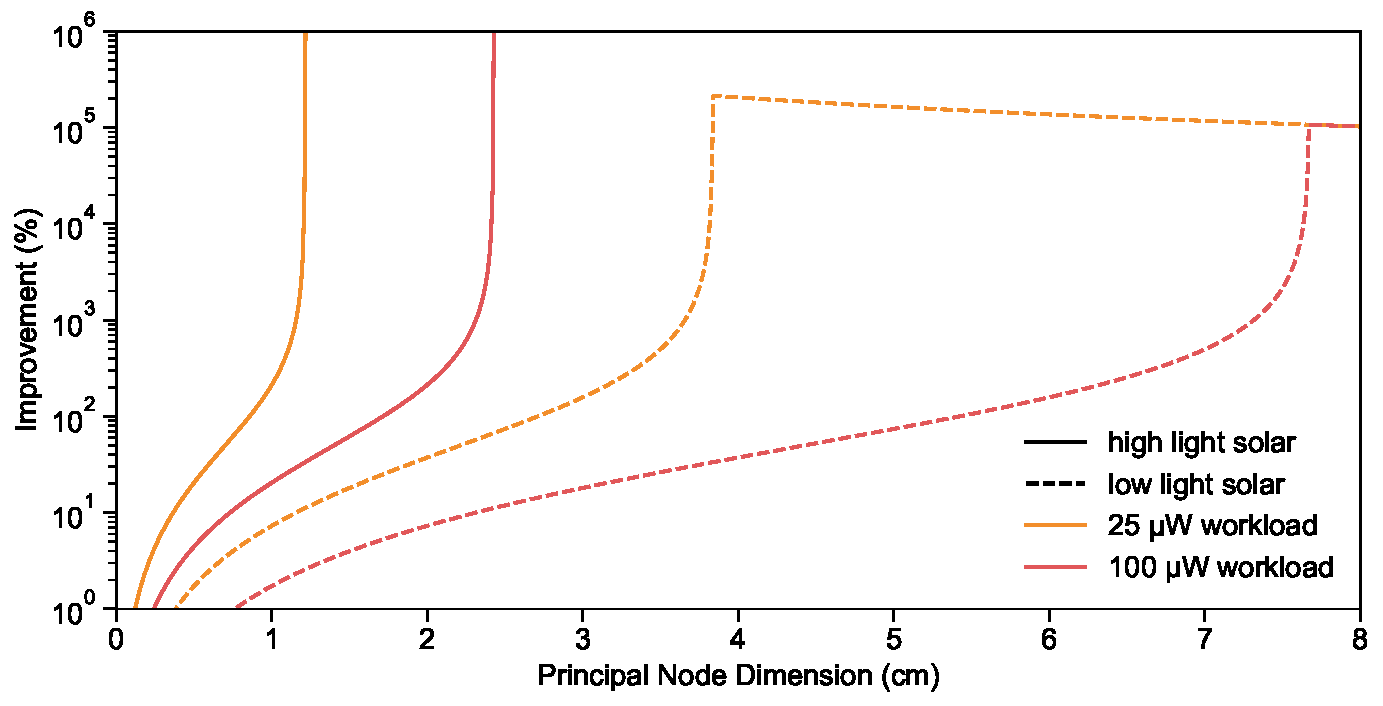
\includegraphics[width=\columnwidth]{figs/primary+harvesting.pdf}
  \caption{
  blah
  }
\end{definefigure}